

\begin{figure}[p]
  \begin{subfigure}[b]{0.5\textwidth}
    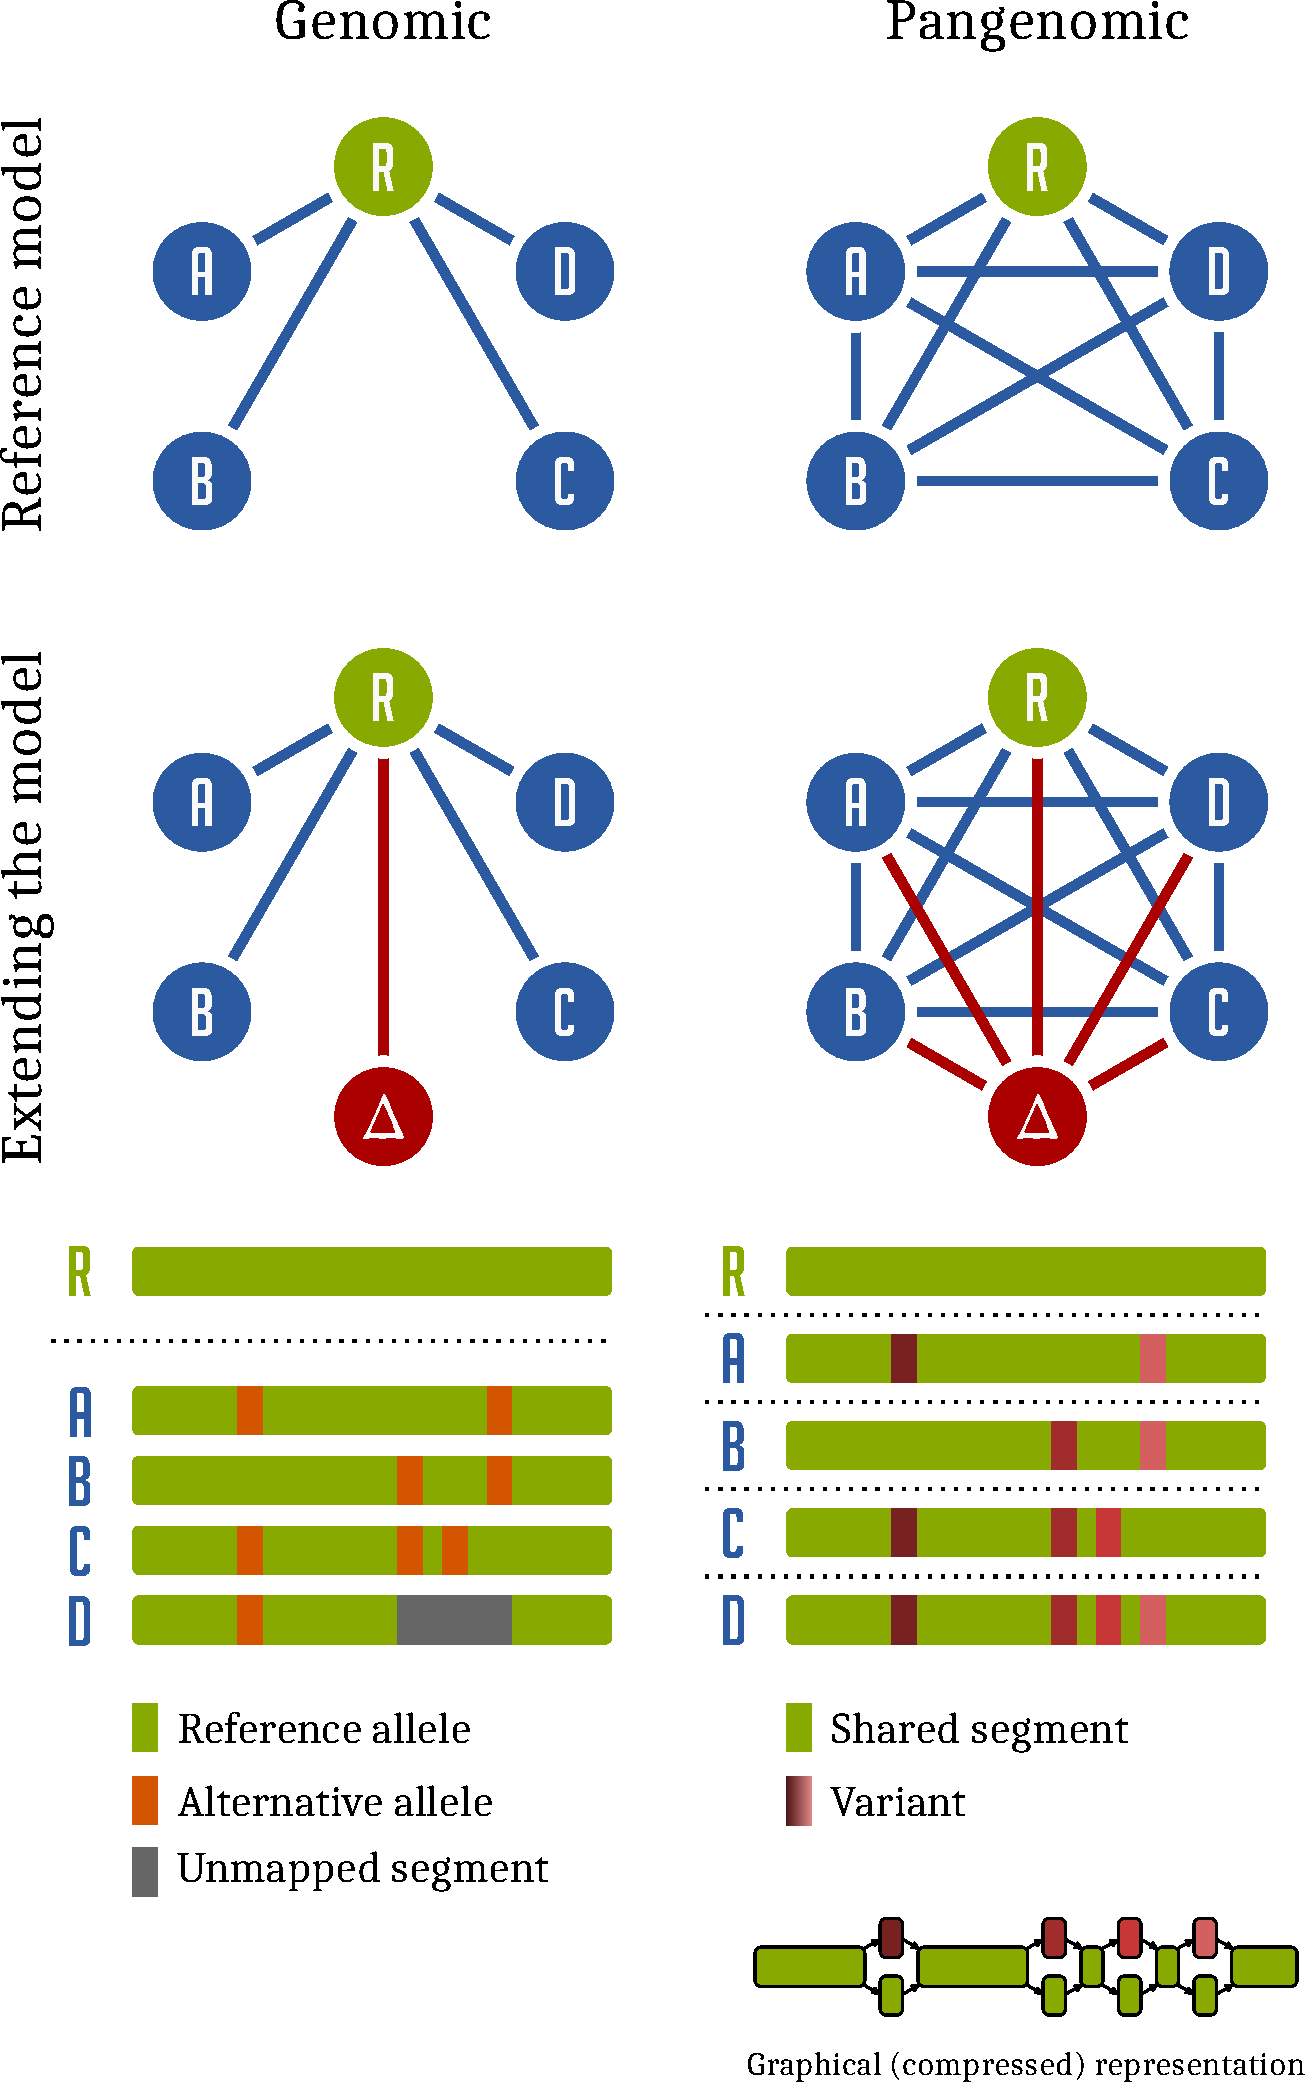
\includegraphics[width=0.9\textwidth]{figures/gen_vs_pang.pdf}
    \centering
    %\caption{}
    %\label{A}
  \end{subfigure}
  \begin{subfigure}[b]{0.5\textwidth}
    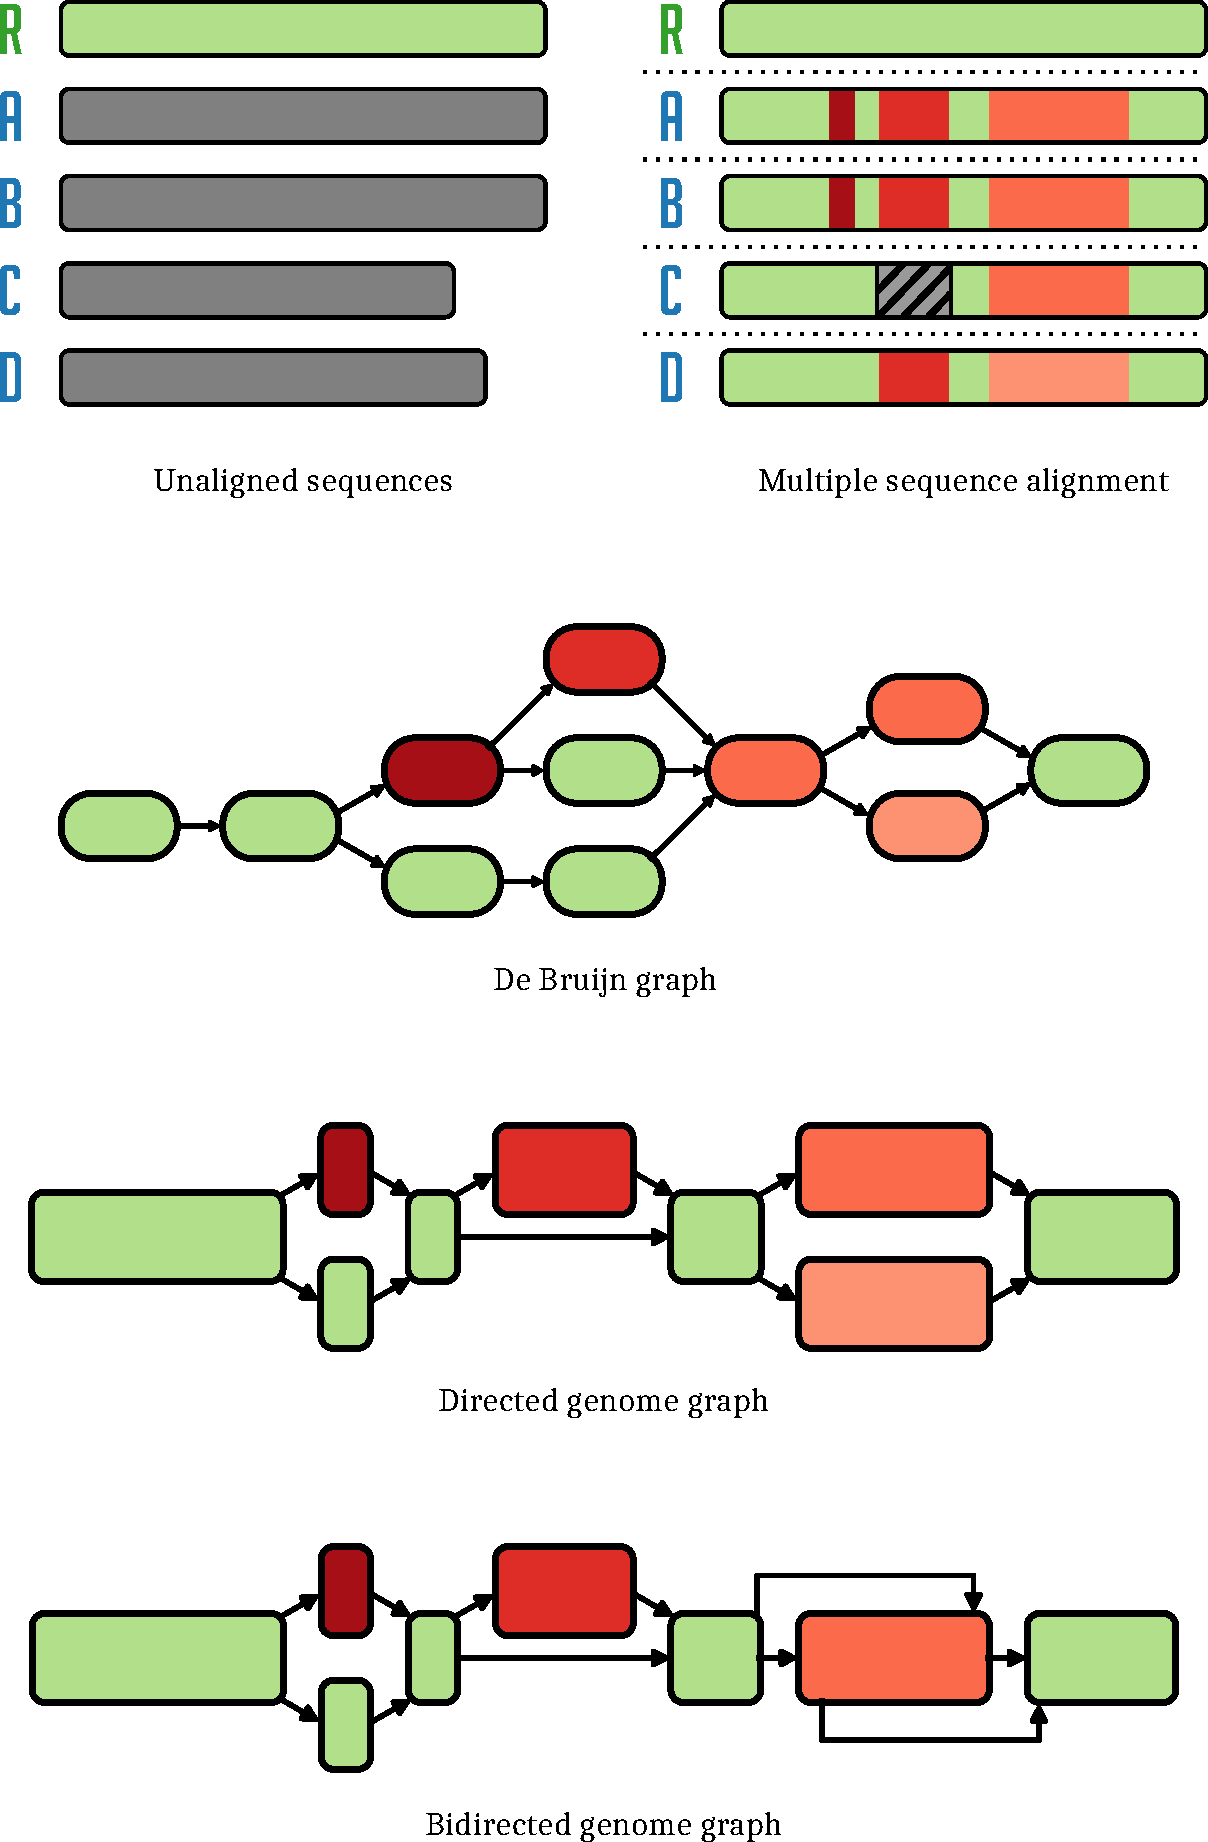
\includegraphics[width=0.9\textwidth]{figures/data_structures.pdf}
    \centering
    %\caption{}
    %\label{B}
  \end{subfigure}
  \\
  \caption{
    \label{fig:models}
    Pangenomic models.
    \emph{Left panel}:
    (top left) In reference based genomic analyses, all genomes ($A \ldots D$) are compared to each other via their relationship to the reference genome $R$.
    (top right) In a pangenomic setting, we attempt to model direct relationships between all the genomes in our analysis, of which a particular reference $R$ is chosen arbitrarily.
    (middle left) When extending our analysis with a new genome, $\Delta$, we add it to the genomic model by comparing it to reference $R$.
    (middle right) In contrast, adding a new genome to a pangenomic analysis compares it directly with all other genomes in the model.
    (bottom left) Regions of some genomes are unalignable against the reference, and cannot be represented in a list of variants.
    (bottom right) A graphical model of the genomes allows direct all-to-all comparison, capturing all of their sequence relationships.
    \emph{Right panel}:
    (top left) A collection of sequences representing a pangenome.
    (top right) Multiple sequence alignment of the sequences captures their mutual relationships.
    (middle top) In a de Bruijn graph, sequences are represented without bias, but variants may correspond to larger graph structures.
    (middle bottom) An acyclic sequence graph is equivalent to the multiple sequence alignment.
    (bottom) A generic sequence graph can represent a structural variant (in orange, right) compactly, using edges between the forward and reverse strands of the graph to indicate the presence of an inversion.
  }
\end{figure}

\begin{figure}[p]
  \begin{minipage}[c]{0.67\textwidth}
    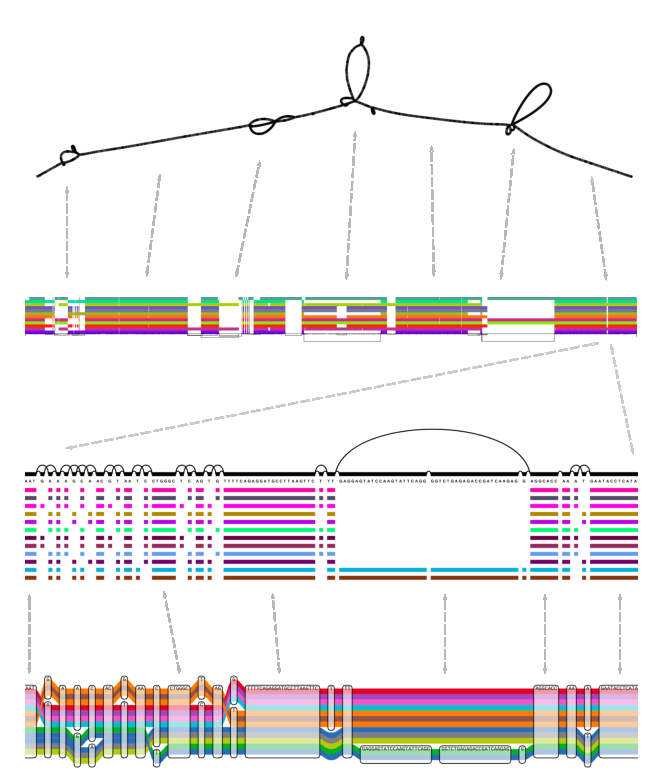
\includegraphics[width=\textwidth]{figures/fig2viz.pdf}
  \end{minipage}\hfill
  \begin{minipage}[c]{0.3\textwidth}
    \caption{
      Visualizing a graph of GRCh38 and its alternate sequences in the gene HLA-DRB1 built with \textsc{VG msga} \cite{Garrison_2019}.
      \emph{Top}: \textsc{Bandage}'s force directed layout reveals large scale structures \cite{Wick_2015}.
      \emph{Top middle}: \textsc{ODGI viz}'s binned, linearized rendering of the paths (colored bars) versus the sequence and topology of the graph (below).
      \emph{Bottom middle}: A fragment of \textsc{VG viz}'s linearized rendering, showing base-level detail.
      \emph{Bottom}: The same fragment rendered with the \textsc{Sequence Tube Map} \cite{Beyer_2019}.
      Dashed lines show correspondence between the visualizations.
    } \label{fig:visualization}
  \end{minipage}
\end{figure}

\begin{figure}[p]
\centering
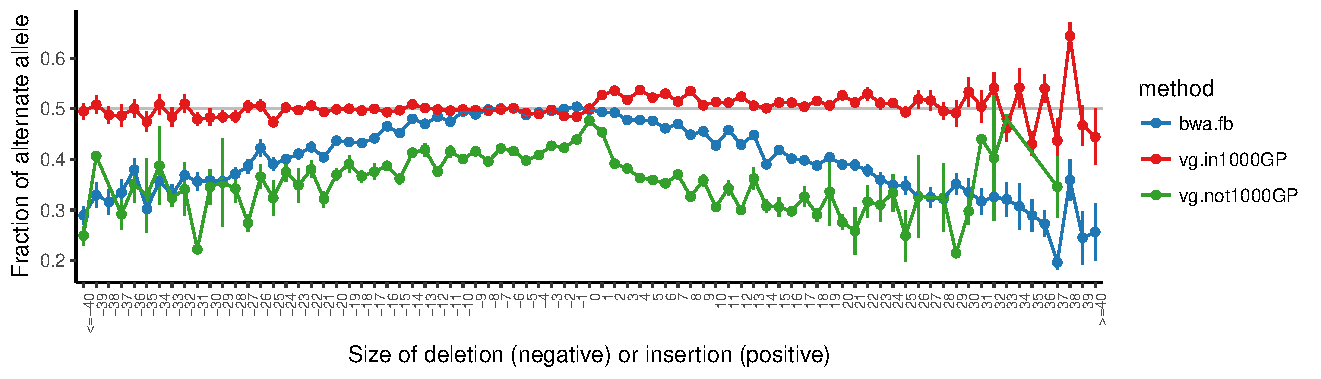
\includegraphics[width=1.0\textwidth]{figures/HG002_wg_pan_ref_bwa_true_hets_allele_balance_tsv_gz_3.pdf}
\caption[Indel allele balance in HG002]{The mean alternate allele fraction at heterozygous variants in HG002/NA24385 validated in the Genome in a Bottle truth set \cite{zook2014integrating} as a function of deletion or insertion size (SNPs at 0).
  Error bars are $\pm$ 1 s.e.m.
  Blue points show the allele balance metric across allele lengths for alignments with \textsc{bwa mem} \cite{Li_2013} and variant calls made by \textsc{freebayes} \cite{garrison2012haplotype}.
  Variant calls were made with alignment to a variation graph built from the 1000 Genomes Project variants \cite{1000_2015}, followed by variant calling in \textsc{VG}.
  These are divided into two groups: calls at variants in the graph used for the alignment (red) and those to variants that are private to HG002 (green).
  Reprinted from \cite{Garrison_2018}.}
\label{fig:allelebalance}
\end{figure}

